\section{Cross-Validation}
Ohne Cross-Validation: Test-Fehler basiert auf 20\% der Daten.\\
Funktionsweise der k-Fold-Crossvalidation: Daten werden zuerst geshuffelt. Anschliessend aufgeteilt in k-Fold (Üblich: 5-Fold, 10-Fold. Gibt aber auch N-Fold wo jeder Fold nur ein Datenpunkt hat). Dann wird jedes mal ein anderer Fold als Test-Datensatz genommen und das Modell trainiert.\\
\textit{Hinweis: Daten in einem Fold ändern sich während den einzelnen Splits nicht. Diese bleiben über die ganzen Trainings gleich. Weiter muss die Preprocessing-Pipeline während den einzelnen Splits laufen und nicht davor, da sonst Ergebnisse verzerrt werden.}
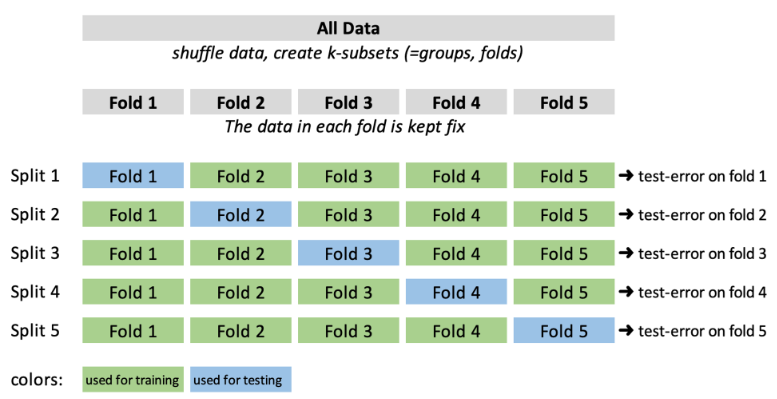
\includegraphics[width=\linewidth]{img/cross-validation.png}
\subsection{Ziel 1: Generalisierungsfehler schätzen}
Hier wird aus den einzelnen Testfehler der Durchschnitt genommen und so der Mean und die Variance des Testfehlers genommen. Ist genauer als mit einzelnen Tests.
\subsection{Ziel 2: Auswahl von Hyperparameter}
Man variert mit den Hyper[arameter (Regularisierungslamda, etc.) und findet so den optimalen Parameter $\lambda_{opt}$ heraus
\subsection{Scikit-learn Cross-Validation}
Einzelne Daten werden vorher ganz rausgenommen als Testdaten. Dann wird mit anderen Cross-Validation gemacht. Wird meist empfohlen.
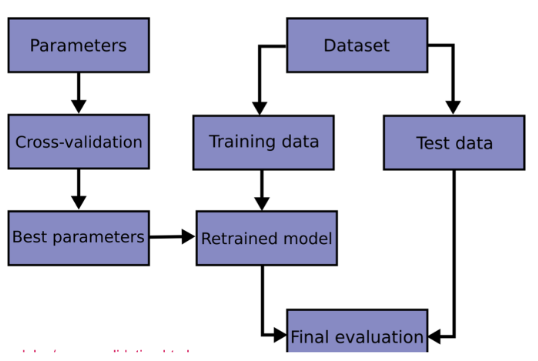
\includegraphics[width=\linewidth]{img/scikit-cross-validation.png}
\section{Artificial Neural Networks}
AI ist inspiriert von unserem Gehirn und den Neuronen. Die biologischen Neuronen wurden vereinfacht in ein Artificial Neuron. Diese bieten ein Input-Vektor. Jedes Neuron hat seine eigenen Input-Gewichte und ein Bias (Intercept). Sie berechnen die Summe von den gewichtenten Inputs (Skalarkprodukt), fügen Bias hinzu und passen es in eine nichtlineare Aktivierungsfunktion. Nachfolgend ein Beispiel eines einfachen Netzes:
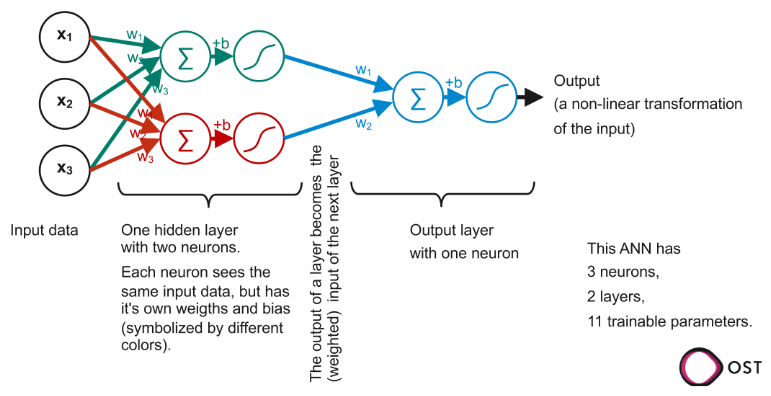
\includegraphics[width=\linewidth]{img/neural-network.png}
Hat ein Netz zahlreiche Hidden Layer, dann wird von einem \textbf{Deep Neural Network} gesprochen.\\
\\
Ein ANN ist eine Datenstruktur zur Definition beliebig komplexer mathematischer Funktionen.
\begin{itemize}
\item ANNs sind aus (vielen) relativ einfachen Ausdrücken zusammengesetzt.
\item Ein ANN ist ein Ausdrucksbaum. Jeder Knoten kann ausgewertet werden.
\end{itemize}

\subsection{ANN trainieren}
\begin{itemize}
\item Wir betrachten einen einfachen Fall von \textbf{supervised learning}: Für jede Eingabe $\vec{x}_i$ erhalten wir die Ausgabe $y_i$ (bekannte Ausgaben werden gewöhnlich als \textbf{Zielwerte} oder \textbf{Labels} bezeichnet)
\item Das ANN wird mit zufälligen Gewichten initialisiert und erzeugt eine Ausgabe $\hat y$. Dann wird ein Optimierer (z. B. SGD) eine Kostenfunktion (z. B. MSE).
\item Das heißt, bei jeder Iteration und für jedes einzelne Gewicht w(und jeden Bias b) wird die partielle Ableitung $\frac{\delta}{\delta w}(y- \hat y)^2$ berechnet werden muss. Glücklicherweise gibt es einen Algorithmus, der dies sehr effizient macht: \textbf{Backpropagation}.
\end{itemize}
